\documentclass[a4paper,11pt,twoside]{article}
%\documentclass[a4paper,11pt,twoside,se]{article}

\usepackage{UmUStudentReport}
\usepackage{verbatim}   % Multi-line comments using \begin{comment}
\usepackage{courier}    % Nicer fonts are used. (not necessary)
\usepackage{pslatex}    % Also nicer fonts. (not necessary)
\usepackage[pdftex]{graphicx}   % allows including pdf figures
\usepackage{listings}
%\usepackage{lmodern}   % Optional fonts. (not necessary)
%\usepackage{tabularx}
%\usepackage{microtype} % Provides some typographic improvements over default settings
%\usepackage{placeins}  % For aligning images with \FloatBarrier
%\usepackage{booktabs}  % For nice-looking tables
%\usepackage{titlesec}  % More granular control of sections.

% DOCUMENT INFO
% =============
\department{Institution för Datavetenskap}
\coursename{Datavetenskapens byggstenar 7.5 p}
\coursecode{DV160HT15}
\title{OU4 Analysis of Complexity}
\author{Lorenz Gerber  ({\tt{dv15lgr@cs.umu.se}})}
\date{2015-12-25}
%\revisiondate{2015-09-15}
\instructor{Lena Kallin Westin / Johan Eliasson}


% DOCUMENT SETTINGS
% =================
\bibliographystyle{plain}
%\bibliographystyle{ieee}
\pagestyle{fancy}
\raggedbottom
\setcounter{secnumdepth}{2}
\setcounter{tocdepth}{2}
%\graphicspath{{images/}}   %Path for images

\usepackage{float}
\floatstyle{ruled}
\newfloat{listing}{thp}{lop}
\floatname{listing}{Listing}


% DEFINES
% =======
%\newcommand{\mycommand}{<latex code>}

% DOCUMENT
% ========
\begin{document}
\lstset{language=C}
\maketitle

\tableofcontents
\newpage

\section{Introduction} 
The aim with this laboration was to apply experimental and asymptotic
complexity analysis of algorithms. This type of experiments and
analysis are used to determine the time or space complexity of an 
algorithm. Or a bit more casual, it is used to find out how a
algorithm behaves for varying input sizes. The analysis seeks to 
answer the question: In which mathematical relation is
the algorithm's runtime to the size of input data. A practical 
example is to describe the needed time for sorting a list, dependent 
on the number of list elements. Such an analysis results in an algebraic
expression, a function $f(n) = t$ where $n$ is the input size and $t$
the algorithm runtime. This will allow to classify algorithms into a
number of groups according to their most dominant term in the 
describing algebraic function: $k, log(n)$, $n$, $n^2$, $n^k$ or $a^n$.

In this laboration, we were working with two common ways for
determining the function relation between input size and runtime:
`experimental complexity analysis' and `asymptotic complexity analysis
based on calculation of primitive operations'. While both of these
methods can yield rather complex expressions, the aim is to find a
simple formula that describes the relation 'on the safe side', i.e. a
conservative estimation of run-time. This last description, finding
a simple, conservative expression for the relation of input size and
runtime qualifies as a `sloppy' definition of the `Big O' notation
which will be described in more detail further down.

\subsection{Experimental Complexity Analysis}
In experimental complexity analysis, the time consumption of the
algorithm is measured for a number of different input sizes. The value
pairs are then visualized in a scatter plot. It is important to choose
apropriate ranges of input size $n$ but also a reasonable number of
replicate measurments for each input size. 
The replication is important for mainly two reasons: First, the 
performance of a computer is not perfectly constant over time. 
It varies within a small range and measurments will
therefore spread somewhat around a theoretical `true' value. Second,
and in most cases more important, many algorithms have a certain
`random' component built in. Alternatively, the test data could be
generated randomly to assess an average case. Taking up the
example of sorting a list again, the data could be already sorted in the
best case or oposite to the requested sort sequence in the worst
case. In any case, replicate measurments for the same input size are
inavoidable.

After plotting the experimental data, assumptions about the relation
between input size and runtime can be done. They can be visually tested
by transforming the experimental data with the inverse of the expected
function. If, for example a graph looks like a second degree polynom,
transforming the response variable with the square-root should yield a
straight line, which visually is much easier to identify as such than
a curve. If the assumption was correct and the resulting graph looks
linear, a linear regression analysis will numerically provide proof
for the assumption. The obtained line equation can then be
transformed back, in the described case resulting in a second degree 
polynom. From here, the next step will be to determine `ordo' of the
obtained function which will be described further down.

\subsection{Asymptotic Complexity Analysis}
In asymptotic complexity analysis, the aim is the same as described
above in experimental complexity analysis: Obtaining a algebraic
relation between input data size and runtime. However, in asymptotic
complexity analysis, the algorithm must be know and available. The
analysis is based on a detailed account for how often each step in the
algorithm will run as a function of input size $n$. There can be
certain steps in an algorithm, that will be independent of input
size, constant. Others will be related linear, polynomal, logarithmic
or exponential with input size. A Typical example is a double
\verb!For! loop: It will yield a $n /times n$ relation, hence it
results in a $n^2$ funtion.

The steps to account for in an algorithm are called 'primtive
operations'. This is a rather theoretical definition that leaves some
room for interpretation. But in general, primitive operations are
\verb![read]!, \verb![write/assign]!, \verb![compare]!,
\verb![increase/decrease]!, \verb![arithmetic operations]! etc. Summing up
all primitive operations for a given algorithm will result in a
function $f(n)$ where $n$ is the input size. Primitve operations will
not perfectly reflect the real case as it can for example not take 
cache optimizations of a given system into account. Already the use of
different compilers for a given source code can result in differences
regarding primitive operations. 

\subsection{The `Big O' notation'}
`Ordo' or `Big O' notation is a mathematical definition of an algorithms'
time complexity. It's formal defintion is shown in equation
(\ref{eq:ordo})\cite[pp. 245]{janlert2000}.  

\begin{equation} \label{eq:ordo}
f(n) \Rightarrow O(g(n)) \textrm{ if } f(n) \leq c \times g(n)
\textrm{ for } n \geq n_{0} \textrm{ and }
c > 0 \textrm{ and } n_{0} \geq 1
\end{equation}

In words: If the function $c \times g(n)$ for $n$ larger than $n_{0}$
is always bigger than $f(n)$, it is of $O(g(n))$ (say: $ordo$  $g$ of
$n$). Hence knowing `ordo' of an algorithm gives a good estimation 
of it's time complexity.

\subsection{Determining of \textit{Ordo}, $c$ and $n_{0}$}
Determing `Ordo' is done in several steps. First the most dominant
function terms of $f(n)$ has to be found and set as $g(n)$. In a
general second degree polynom, $n^2$ is for example the dominant term.

Then the constant factor $c$ is determined by calculating the limes
from n to infinity of dividing $f(n)$ by $g(n)$ according to
equation (\ref{eq:limes}).  

\begin{equation} \label{eq:limes}
\lim_{n \to \infty} {f(n) \over g(n)} + 1
\end{equation}

The value $n_{0}$ is the lower limit of input size $n$ for which
$g(n)$ will be at least equal or larger than $f(n)$. It is found by
solving equation \ref{eq:nzero}. 

\begin{equation} \label{eq:nzero}
c\times g(n) = f(n)
\end{equation}


\section{Material and Methods}

\subsection{Experimental Complexity Analysis}
We obtained a compiled program to run from the command line. The
program would take three arguments: a selector for one of two
implemented algorithms, size of in data and number of repetitions. It
was unknown to us which algorithms were implemented in the
program. The program would run a certain time and before quitting, 
print the runtime to standard out.

To automate the experimental process, a shell script (listing \ref{ls:bash}) 
was written that run the program 10 times for the input sizes n = (1'000, 
2'500, 5'000, 10'000, 15'000, 20'000, 25'000, 50'000, 75'000, 100'000,
125'000, 150'000, 200'000).

\begin{listing}

\begin{verbatim}
#!/usr/local/bin/bash                                                                                           
ARRAY=(10000 15000 20000 25000 50000 75000  100000 125000 150000 200000)
for a in ${ARRAY[*]}
do
    for b in {1..10}
    do
        ./algorithms_osx -2 $a
    done
done
\end{verbatim}
\caption{Shell script to automate the collection of experimental
  data. Standard output was piped and appended to a text file.\label{ls:bash}}
\end{listing}

The script was run from the bash commandline on a MacbookPro8,1 and
the output piped and appended to a text file which was then imported
to statistical computing environment R \cite{rlanguage}. All data analysis and
plotting was done in R. 


\subsection{Asymptotic Complexity Analysis}
We were given pseudo code of a bubble sort algorithm (listing \ref{ls:bubble})
to conduct asymptotic complexity analysis. A short description on how
to account for primitive operations was available through the course
homepage \cite{complex}.

\begin{listing}
\begin{verbatim}
Algorithm bubbleSort(numElements, list[])
input:  numElements, the number of elements in the list
        list, a list of numbers to be sorted
output: the sorted list

1:  done <- false
2:  n <- 0
3:   while (n < numElements) and (done = false)
4:      done <- true
5:      for m <- (numElements -1) downto n
6:          if list[m] < list[m - 1] then
7:              tmp <- list[m]
8:              list[m] <- list[m - 1]
9:              list[m - 1] <- tmp
10:             done <- false
11:    n <- n + 1
12: return list 
\end{verbatim}
\caption{The given pseudo code of a bubble sort.}
\end{listing}

After accounting for primitive operations and obtaining algebraic
functions describing `best' and `worst' case for the bubblesort algorithm, 
`ordo' expressions were determined according to lecture notes. 


\section{Results}
\subsection{Experimental Complexity Analysis}

\begin{figure} 
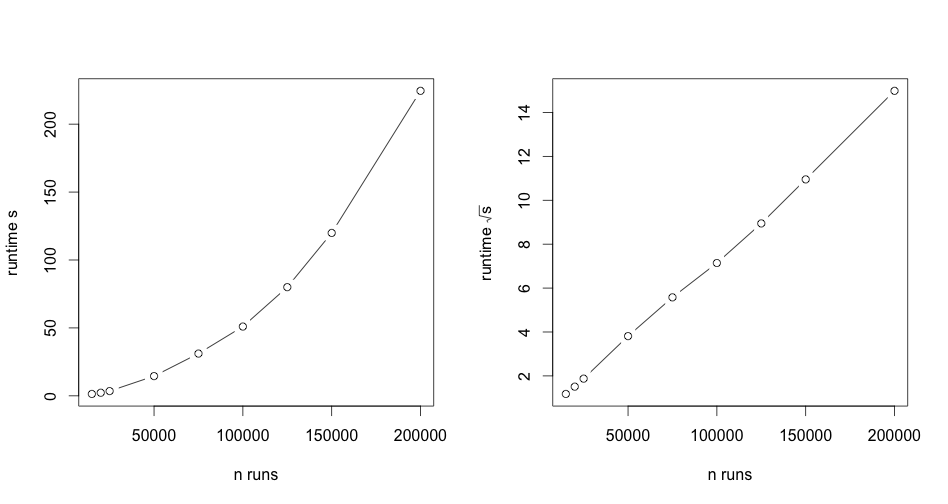
\includegraphics[width=\textwidth]{graph1.png}
\caption{\textit{Runtime values in seconds for a series of \textit{n}
  repetitions of the investigated algorithm. The left panel shows the
  measured times. For the right panel, the square root for each time
  value was calculated before plotting.}\label{ls:bubble}}
\label{fig:graph}
\end{figure}

The left panel of figure \ref{fig:graph} shows the experimental
runtime values plotted against $n$ length of input data. The values
were then transformed by calculating the square root. The 
transformed data is shown in the right panel of figure 
\ref{fig:graph}. Then linear regression was calculated on the
transformed data (\textit{table\ref{tab:regression}}).

\begin{table}[]
\caption{\textit{Linear regression of the transformed experimental data}}
\label{tab:regression}
\begin{tabular}{lll}

gradient &  & $7.348 \times 10^{-5}$ \\
intercept &  & $1.393 \times 10^{-2}$ \\
$R^2$ &  & 0.9988 \\ 
\end{tabular}
\end{table}

The obtained linear equation was transformed back to yield a
quadratic function as shown in equation (\ref{eq:quadratic}).

\begin{equation} \label{eq:quadratic}
y = 5.4 \times 10^{-9}x^2 + 2.1 \times 10^{-6}x + 0.2 \times 10^{-4}
\end{equation}

Then $c$ was determined according to equation (\ref{eq:limes}) and
$n_0$ was determined by solving the quadratic equation resulting from
$f(n) = g(n)$ (Table \ref{tab:ordo}, figure \ref{fig:ordo}). 

\begin{table}[]
\caption{\textit{Calculated value for ordo determination}}
\label{tab:ordo}
\begin{tabular}{lll}
$c$                       &  & $6.4 \times 10^{-9}$ \\
\multicolumn{1}{c}{$n_0$} &  & 2060                
\end{tabular}
\end{table}


\begin{figure} 
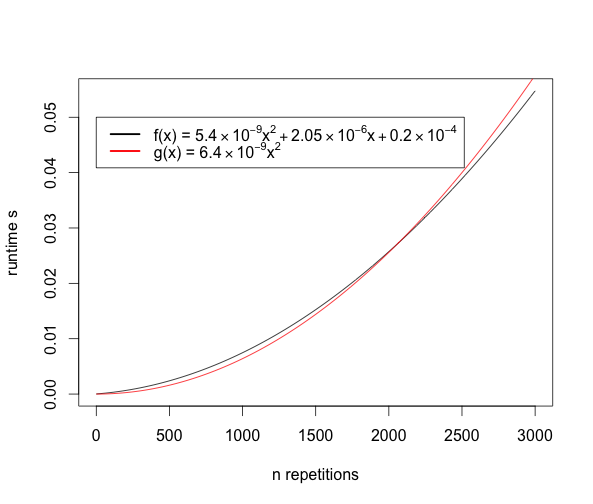
\includegraphics[width=\textwidth]{ordo.png}
\caption{\textit{Comparison of $f(x)$ and $O(g(x))$ in the range of $n_{0}$
  which was determined to be at about $n = 2600$.}}
\label{fig:ordo}
\end{figure}

\subsection{Asymptotic Complexity Analysis}
\subsubsection{Worst Case}
Listing \ref{ls:worst} shows the determination of primitive operation
for the `worst' case. The line numbers correspond to the line numbers
in the original pseudocode shown in listing \ref{ls:bubble}.

\begin{listing}
\begin{verbatim}

1:  1 * [<-] + 
2:  1 * [<-] + 
3:  (numElements + 1) * 
    (3 * [get] + 1 * [<] +  1 * [=] + 1 * [AND]) + 
4:  numElements * (1 * [<-]) +
5:  init:
    (numElements * (numElements -1) / 2 + 1) *
    (1 * [get] + 1 * [-] + 1 * [<-]) +
 
    cond success + counter: 
    numElements * (numElements - 1) / 2) *
    (2 * [get] + 1 * [>] + 1 * [--]) +

    cond fail:
    numElements * 
    (2 * [get n] + 1 * [>]) +

6:  (numElements * (numElements - 1) / 2) * 
    (2 * [get] + 2 * [list[]] + 1 * [-] + 1 * [<] + 
7:      1 * [get] + 1 * [list[]] + 1 * [<-] +
8:      1 * [get] + 1 * [-] + 1 * [list[]] + 1 * [<-] + 
9:      2 * [get] + 1 * [-] + 1 * [ <-] +
10:     1 * [<-] ) +
11: numElements * (1 * [get] + 1 * [+] + 1 * [<-] +
12: 1 * return

set numElements = x

1:  1 + 
2:  1 + 
3:  (x + 1) * 6  
4:  x * 1
5:  (x * (x-1) / 2 + 1) * 3 +
    (x * (x - 1) / 2) * 4 +
    x * 3 +
6:  (x * (x - 1) / 2) * (6 +
7:    3 + 
8:    4 +
9:    4 + 
10:   1) + 
11: x * 3 +
12: 1 

Hence:
1 + 1 + 6x + 6 + x + 1.5x^2 - 1.5x + 3 + 2x^2 - 2x + 
3x + 9x^2 - 9x + 3x + 1

= 12.5x^2 + 4.5x + 12

\end{verbatim}
\caption{\textit{Determining the `worst case' complexity for the given
    `bubblesort' algorithm. The line numbers correspond to those in 
listing \ref{ls:bubble}}.\label{ls:worst}}
\end{listing}

\subsubsection{Best case}
Listing \ref{ls:best} shows the determination of primitive operation
for the `best' case. The line numbers correspond to the line numbers
in the original pseudocode shown in listing \ref{ls:bubble}.

\begin{listing}
\begin{verbatim}
1:  1 * [<-] +
2:  1 * [<-] +
3:  2 * (3 * [get] + 1 *[<] + 1 * [and] + 1* [==]) +
4:  1 * [<-] +
5:  init:
    1 * [get] + 1 * [-] + 1 * [<-] +

    cond success + counter:
    (numElements - 1) * (1 * [get] + 1 * [>]) + 1 * [--]) +
    
    cond fail:
    1* [get] + 1 * [>] + 
6:  (numElements - 1) * 
    (2 * [get] +  2 * list[] + 1 * [-] + 1 * [<]) +
11: 1 * [get] + 1 * [+] + 1 * [<-]
12: 1 * [return]

set numElements = x

1:  1 +
2:  1 +
3:  2 * 6 +
4:  1 +
5:  3 + 
    (x - 1) * 3 +
    2 +
6:  (x - 1) * 6 +
11: 3 +
12: 1 

Hence:
1 + 1 + 12 + 1 + 3 + 3x - 3 + 2 + 6x -6 + 3 + 1
= 9x + 15

\end{verbatim}
\caption{Determining the `best case' complexity for the given
  `bubblesort' algorithm. The line numbers correspond to those in
  listing \ref{ls:bubble}.\label{ls:best}}
\end{listing}

In table \ref{tab:ordo2} the keyfigures of the `ordo' determination for
`best' and `worst' case expressions can be found. 

\begin{table}[]
\caption{\textit{Determination of $ordo$ for `Best' and `Worst Case'}}
\label{tab:ordo2}
\begin{tabular}{llcc}
&  & Worst Case & Best Case \\ 
\hline
$f(n)$ &  & \multicolumn{1}{c}{$12.5n^2+4.5x+12$} & \multicolumn{1}{c}{$9x+15$} \\
$g(n)$ &  & \multicolumn{1}{c}{$n^2$}             & \multicolumn{1}{c}{$x$}   \\
$c$    &  & 13.5                                  & 10                          \\
$n_0$  &  & 7                                     & 15                          \\                         
\end{tabular}
\end{table}

\section{Discussion}
\subsection{Experimental Complexity Analysis}
Plotting the experimental data (left panel of figure \ref{fig:graph}) showed that
the investigated algorithm is not of $O(k)$ or $O(n)$ as this would
have yielded a straight line. To test the hypothesis whether the
algorithm could follow a second degree polynom function, the response
variabel was transformed. If the hypothesis is true, one can expect
the resulting plot to expose linear behaviour. As can be seen in the
right panel of figure \ref{fig:graph}, this was the case. At least
visually, the obtained data looked linear. To get a more objective
metric, linear regression was calculated on the transormed data. The
obtained $R^2$ value of 0.9988 is a very strong indication that the
transformed data is well represented by a linear equation 
(table \ref{tab:regression}). So the hypothesis that the obtained
experimental data follows a second degree polynom function was
seen as proven and the linear regression equation was transformed back
to yield a second degree polynom function (equation
\ref{eq:quadratic}). Finally, $c$ and $n_{0}$ were calculated to confirm
the validity of the found `ordo' defintion (table \ref{tab:ordo}). 


\subsection{Asymptotic Complexity Analysis}
The main flow structural feature of the given bubble sort algorithm can be
described as a \verb!for! loop encapsulated in a \verb!while!
loop. 

\subsubsection{Worst Case}
The `worst' case occurs, when the in-data list is sorted in the
oposite direction. Only by looking at the above described encapsulated
loop structure, it becomes clear that the complexity will be at least
$n \times n$, hence $n^2$. However, by reducing the inner loop in
every additional round for the outer loop to skip already sorted
elements, the inner loop runs in the worst case just roughly ${n /over
  2}$ times. All further details can be seen in listing
\ref{ls:worst}. In brief, it was chosen to also account one primitive
operation for each \verb!read! of a variable.

After finding the $f(n)$, `ordo' was determined. $c$ was calculated
according to equation \ref{eq:limes} and $n_{0}$ by solving equation
\ref{eq:nzero}. 

\subsubsection{`Best Case'}
The best case occurs when the in-data list is already sorted. In this
case, the outer \verb!while! loop will run through just once while the
inner \verb!for! loop will run about $n-1$ times where $n$ is the
number of elements. However, on each \verb!for! loop round, just a
part of the code will be executed, as the \verb!if! condition will
always evaluate to \verb!false!. Hence, at `best' case, the given
bubble sort algorithm can be expected to be of linear time complexity
which was also the result of summing up the primitive operations as
shown in listing \ref{ls:best}.  

Determination of `ordo' was accomplished in the same way as for the
`best' case as described earlier. The result is shown in table
\ref{tab:ordo2}.

\section{Reflections on the laboration}
I enjoyed solving the present laboration. From the first part I liked
the practical aspect of doing data analysis, interpreting experimental
data and coming up with a function describing the data. I found the 
laboration well explained and on an appropriate level of difficulty. 

In the asymptotic complexity analysis I was surprised how much time
once could spend on a rather simple and short algorithm and still time
after time finding again inconsitencies in how one assigned primitive
operations. It took me at least five attempts to get the final version
of the `worst' case analysis. Altough the final result did not change
much from attempt to attempt, it felt just wrong to not justify small
inconsistencies as I thought every time it would be the last.


\addcontentsline{toc}{section}{\refname}
\bibliography{references}

\end{document}
